%% ----------------------------------------------------------------
%% Article.tex
%% ---------------------------------------------------------------- 

%% You mostly won't have to worry about this file

\documentclass{ecsarticle}     % Use the Article Style
%\documentclass{IEEEtran}
\graphicspath{{Figures/}{../Figures/}}   % Location of your graphics files
\usepackage{natbib}            % Use Natbib style for the refs.
\usepackage{lipsum}
\usepackage{todonotes}
\usepackage{multirow}
\usepackage{longtable}
\usepackage{array}
\newcommand{\inote}[1] {\todo[inline]{#1}}
\removecolourlinks    % Uncomment this command to remove colour from any links
%\input{Definitions}            % Include your abbreviations
%% ----------------------------------------------------------------


\begin{document}
\frontmatter
\title      {ELEC6089 High Voltage Insulation Systems Assignment 1}
\authors    {\texorpdfstring{\href{mailto:tjs1g10@ecs.soton.ac.uk}{Thomas J. Smith}}{Thomas J. Smith}, 
\texorpdfstring{\href{mailto:dm4g10@ecs.soton.ac.uk}{David Mahmoodi}}{David Mahmoodi},
\texorpdfstring{\href{mailto:bh8g10@ecs.soton.ac.uk}{Brendan Hickman}}{Brendan Hickman}, 
\texorpdfstring{\href{mailto:pplf1g10@ecs.soton.ac.uk}{Patrick P. L. Fong}}{Patrick P. L. Fong}}
%\department  {Electronics and Computer Science}
\group       {HV AC 275kV Bushing Design}
%\addresses  {\groupname\\\deptname\\\univname}
\addresses  {\univname}
\date       {\today}
\subject    {}
\keywords   {}
\maketitle
\begin{abstract}
\lipsum[1]
Hello a
\end{abstract}
%\tableofcontents
%\listoffigures
%\listoftables

%% -----------------------
%% lstpatch.sty
%% -----------------------
%% lstpatch cannot be distributed with these files. I believe it is only needed if the
%% \lstlistoflistings is used. So this has been turned off by default. Re-add if required:
%% \usepackage{lstpatch}
%% \lstlistoflistings
%% You will need to download lstpatch, possibly from:
%% http://web.mit.edu/texsrc/source/latex/listings/lstpatch.sty
%% -----------------------



%\listofsymbols{ll}{$w$ & The weight vector}
\mainmatter
\section{Introduction}
A brief review on field design in HV equipment. This is a sample citation \cite{kuffel2000high}.

Example of~\eref{eq:equation1}.
\begin{equation}
y = ax^2 + bx + c
\label{eq:equation1}
\end{equation}


\tref{Table:tabex} illustrates a table.
\begin{table}[!htb]
  \centering
\caption{The Results}
  \begin{tabular}{cc}
  \toprule
  \textbf{Training Error} & \textbf{Testing Error}\\
  \midrule
  0 & $\infty$\\
  \bottomrule
  \end{tabular}
  \label{Table:tabex}
\end{table}

\lipsum
\section{Overview of Grading Methods}
Electric field stress control is important in the design of many power system elements, especially cable terminations and bushings \cite{james2008condition}.
Failure of a bushing can damage the power transformer it is protecting, which can be an expensive mistake \cite{warne2005newnes}.
Bushings are required to withstand Electrical, Mechanical and Thermal stresses as defined in the IEEE standard C57.19.00 \cite{1440990}.
The design of the bushing is largely determined by the insulation material chosen and the resolution of these conflicting sources of stress.
A good bushing design has insulation that can withstand the applied voltage and thermal characteristics appropriate for the current carried by the conductor \cite{harlow2004electric}.

The problem grading methods attempt to resolve is laid out in figure \ref{figure:problem}.
The grounded transformer casing is shown in light grey which is perpendicular to the the bushing insulation shown in dark grey and the high voltage conductor in white.
The top of the bushing is exposed to air, while the other side is exposed to transformer oil.
Conducting a numerical analysis or simulation would show that the conductor surface within the plane of the transformer casing and at the points marked by red crosses would experience high electric field stress.
The bushing insulation is designed to withstand the high electric field between the conductor and the transformer casing, however at the points marked with crosses the interface between the solid insulation and the air/transformer oil would cause surface discharge leading to relatively low flashover voltages \cite{kuffel2000high}.
It is therefore necessary to develop methods of reducing electric field stress to a more uniform distribution for both functional purposes and the economic use of space and materials \cite{james2008condition}.

\begin{figure}[!h]
   \centering
   \includegraphics[width = 0.7\textwidth]{GenericBushing.pdf}
   \caption{The Bushing Problem}
   \label{figure:problem}
\end{figure}

\subsection{Low Voltage and DC Solutions}
There are several methods that can be used dependant upon the application.
Low voltage solutions include internal and external screening electrodes, while resistive stress control can be used for DC applications.
\inote{TS - I can't find any good references for these types, only his notes and the hst.tu notes seem to cover it and then it is just lecture slides, not a credible resource like a book or something}

\subsection{Capacitive Grading}
Capacitive grading was first proposed by R.Nagel of Siemens in a German paper published in 1906 \cite{harlow2004electric}.
The value of this type of arrangement was quickly recognised, and is now industry standard practice for AC bushing designs for 25kV - 1500kV applications \cite{james2008condition}.
The general concept of the design is illustrated in figure \ref{figure:fieldgeneric}, showing the isolated foils inserted inside the solid bushing insulation.
Shown in red in figure \ref{figure:fieldgeneric} is the potential field with no grading, and in blue with the isolated conductive foils inserted.
It shows that the whole dielectric is much more evenly stressed with the capacitive grading method.
\begin{figure}[!h]
   \centering
   \includegraphics[width = 0.7\textwidth]{BushingFieldDiagram.pdf}
   \caption{Field Distribution both without capacitive grading (shown in red) and with capacitive grading (shown in blue), modified from \cite{james2008condition}}
   \label{figure:fieldgeneric}
\end{figure}

The insulation is stressed in both a radial and axial direction, which sum to give the tangential field.
The radial component $E_r$ can cause breakdown of the insulating material, while the axial component $E_z$ can cause surface discharge along the boundary \cite{Ahmed11}.
These can be seen in green in figure \ref{figure:fieldgeneric}.
These sum up to give the tangential field $E_t$.

The most widely used method used to choose the dimensions and locations of the foils is double sided capacitive grading, of which there are two variants \cite{Ahmed11}.
Before the distinction is made between the two, it is first necessary to introduce some terms.
\begin{figure}[!h]
   \centering
   \includegraphics[width = \textwidth]{GradingSymbols.pdf}
   \caption{Symbols for calculating capacitive grading, modified from \cite{Ahmed11}}
   \label{figure:fieldgeneric}
\end{figure}
Firstly, The radius of the foil referenced from the centre of the conductor is termed $r_n$. 
The spacing between each foil is defined in equation \ref{eq:Spacing}.
\begin{equation}
   \label{eq:Spacing}
   S_n = r_n - r_{n-1}
\end{equation}
Additionally, the length of each foil is referred to as $l_n$ and the difference in length on the right and left side between each foil is termed $b_{ln}$ and $b_{rn}$. 
Symmetric double sided capacitive grading is achieved when $b_{ln}=b_{rn}$ \cite{Ahmed11}. 
The total number of foils in the system is $N$.
Also note that subscript $n$ denotes the outermost foil.

The radial spacing and dimension of each foil is determined in the following derivation, which has been verified and modified from \cite{kuffel2000high}.
When a conductor is surrounded by concentric foils of dielectric constant $\epsilon$ that is much greater than $\epsilon_{0}$, the system can be treated as a set of coaxial cylindrical capacitor units connected in series.
In this derivation, the simplest boundary condition is assumed, that is the mean value of the radial field $E_r$ remains constant within the foils.
The foils are assumed to be of equal thickness, denoted by $\delta$.
Each of the foils forms a coaxial capacitor stressed by the equal voltage $\Delta V = E_{r}\delta$ providing all capacitances are equal.
The capacitance of each foil is equal providing $C_n = C_{n-1} = C_0$ where equation \ref{eq:Cn} gives the value of each capacitance.
\begin{equation}
   \label{eq:Cn}
   C_n = \frac{2\pi\epsilon l_{n-1}}{ln(\frac{r_{n-1}}{r_{n}})}
\end{equation}

This can be expanded as in equation \ref{eq:lengthequals}.
\begin{equation}
   \label{eq:lengthequals}
   \frac{l_n}{ln(\frac{r_{n-1}}{r_{n}})} = \frac{l_{n-1}}{ln(\frac{r_{n-2}}{r_{n-1}})} = \frac{l_1}{ln(\frac{r_{0}}{r_{1}})}
\end{equation}

An approximate solution for thin foils can then be found.
Under the thin foil assumption, $r_{1} = r_{0} + S_n$ and $\frac{\delta}{r_n}<<1$ even for the smallest radii of the inner conductor.
Equation \ref{eq:simplify} allows the simplification of equation \ref{eq:lengthequals} to equation \ref{eq:simplefoils}.

\begin{equation}
   \label{eq:simplify}
   ln(\frac{r_n}{r_{n-1}}) = ln\frac{1}{1-(\frac{\delta}{r_n})} \approx \frac{\delta}{r_n}
\end{equation}

\begin{equation}
   \label{eq:simplefoils}
   l_{n}r_{n} \approx l_{n-1}r_{n-1} \approx \dots \approx l_{0}r_{0}
\end{equation}

The two methods for solving the recursive equation in equation \ref{eq:simplefoils} is through either radial or axial grading \cite{Ahmed11}.
In radial grading, the spacing of the foils $S_n$ is assumed to be constant. 
This means the length of the foils decreases as it it approaches the outer foils of the bushing.
Equation \ref{eq:evenspace} gives the method to calculate $S_n$ which can then be used in the recursive equation \ref{}, which is a simple form of equation \ref{eq:simplefoils}.
\begin{equation}
   \label{eq:evenspace}
  S_n = \frac{Outer Diameter - Conductor Diameter}{N-1}
\end{equation}

\begin{equation}
   \label{eq:evenspace}
  l_{n+1}= l_{n}\frac{r_{n}}{r_{n} + S_{n}}
\end{equation}

In the axial grading method, the length of each foil is assumed to decay by a constant value with each foil, and the radius at which it is placed is determined by a similar iterative formula.
Radial grading better suits the purposes of this paper, since there is no requirement to assume the length of the final foil.

\section{Capacitive Grading Techniques}
Capacitive graded bushings, sometimes referred to as the field stress-controlled bushing or capacitor bushing \cite{kuffel2000high}, contain concentric conductive foils within the insulation.
Each foil is isolated from the others \cite{Ahmed11}.
By designing the length and radial spacing of these foils, the electric stress and voltage drop in the core along its surface is determined by the ratio of partial capacitances between the foils \cite{Ahmed11}.
The difference between a standard solid bushing and a field stress-controlled bushing is shown in figure \ref{Figure:typesofbushing}.

\begin{figure}[!htb]
  \centering
  \subfigure[Solid Bushing]{
    \includegraphics[height = 6cm]{GenericBushing.pdf} 
	\label{Figure:standardbush}
  }
  \subfigure[Field Stress-controlled Bushing]{
    \includegraphics[height = 6cm]{GenericGradedBushing.pdf} 
	\label{Figure:gradedbush}
  }
\caption{This shows the difference in construction between the two bushing types}
  \label{Figure:typesofbushing}
\end{figure}




\section{Design Details}
The reference model for this project is shown in figure \ref{figure:refproblem}. 
The reference design is a paper impregnated with oil bushing with 21 aluminium foils of $100\mu m$.
One side of the bushing is exposed to air, the other to oil, similar to a transformer bushing.
The diameter of the conductor is 100mm, the bushing diameter is 300mm.
The length of the first foil is 5000mm long, and fixed 2mm into the bushing at the conductor voltage.
The outer foil is also set 2mm inside the bushing and is directly connected to the earthed flange.
The conductor is used at 275kV AC voltage, and the design is known to be flawed.
\begin{figure}[!h]
   \centering
   \includegraphics[width = 0.7\textwidth]{ReferenceDiagram.png}
   \caption{The reference problem taken from \cite{Chen14}}
   \label{figure:refproblem}
\end{figure}

A Matlab script was developed to take a required number of foils, and the inner and outer dimensions of the bushing, to calculate the radial location and length of each foil using the radial grading method as described in section \ref{ss:CapacitiveGrading}.
This script was built to be easily customisable for any number of foils and any initial values, to cater for the calculation of improved designs.
It automatically outputs data in a form for direct input into the COMSOL model, and auto-updates a \LaTeX  file containing the data in table \ref{table:radialvals21}.
Finally, the script plots the calculated foil positions in a crude graph shown in figure \ref{Figure:Both21plots}.
Particularly in figure \ref{Figure:21plot2} the decay shape can be observed as expected.
This allows a quick verification of the scripts accuracy before proceeding to simulation.

\begin{table}[!htb]
\caption{Radial Grading Calculations Results}
\label{table:radialvals}
\begin{center}
\begin{tabular}{cc}
\toprule
\textbf{Radius(mm)} & \textbf{Length(mm)} \\ \toprule
52.00 & 5000.00 \\ 
56.80 & 4577.46 \\ 
61.60 & 4220.78 \\ 
66.40 & 3915.66 \\ 
71.20 & 3651.69 \\ 
76.00 & 3421.05 \\ 
80.80 & 3217.82 \\ 
85.60 & 3037.38 \\ 
90.40 & 2876.11 \\ 
95.20 & 2731.09 \\ 
100.00 & 2600.00 \\ 
104.80 & 2480.92 \\ 
109.60 & 2372.26 \\ 
114.40 & 2272.73 \\ 
119.20 & 2181.21 \\ 
124.00 & 2096.77 \\ 
128.80 & 2018.63 \\ 
133.60 & 1946.11 \\ 
138.40 & 1878.61 \\ 
143.20 & 1815.64 \\ 
148.00 & 1756.76 \\ 
\bottomrule
\end{tabular}
\end{center}
\end{table}


\begin{figure}[!htb]
  \centering
  \subfigure[Wide View]{
    \includegraphics[height = 6cm]{../Matlab_Calculations/RadialGrade21ProfileWide.eps} 
	\label{Figure:21plot1}
  }
  \subfigure[Real Perspective]{
    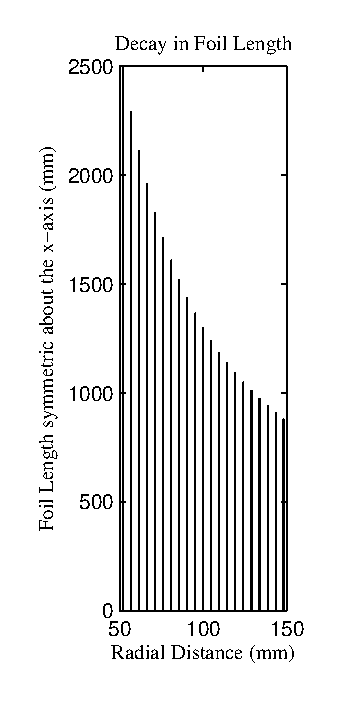
\includegraphics[height = 6cm]{../Matlab_Calculations/RadialGrade21ProfileSquash.eps} 
	\label{Figure:21plot2}
  }
\caption{Representation of foil radial position and length}
  \label{Figure:Both21plots}
\end{figure}

The final information required to be able to proceed to the simulation phase is the relative permittivity of each material.
This was gathered from \cite{Ahmed11} and is shown in table \ref{table:perm}.

\begin{table}[!htb]
\caption{Relative Permittivity of Materials}
\label{table:perm}
\begin{center}
\begin{tabular}{cc}
\toprule
\textbf{Material} & \textbf{Relative Permittivity ($\epsilon_r$)} \\ \toprule
Air & $1$ \\
Oil &$ 2.2$ \\
Paper Impregnated with Oil &$ 4$ \\
Aluminium & $10^8$\\
\bottomrule
\end{tabular}
\end{center}
\end{table}


%  Field_Modelling.tex
% !TeX spellcheck = en_GB
% !TeX root = ReportMain.tex

\section{Modelling Results}
The following simulations were completed using the COMSOL multiphysics software package.
COMSOL is a professional finite element simulation package able to model a variety of physical features.
The following models are created using the AC/DC module, which is used to simulate electric and magnetic fields \cite{ComsolACDC}.
Specifically, the electrostatics interface is used. 
This solves a charge conservation equation for a given voltage and spacial distribution of charge \cite{ComsolACDC}.

\subsection{Finite Element Methods (FEM)}
There are inherent difficulties in solving the partial differential equations that govern many practical engineering problems \cite{kuffel2000high}.
Despite knowing the equations and appropriate boundary conditions that govern a problem, many are complicated by irregular geometries or other discontinuities.
Numerical methods allow approximate solutions to be obtained for problems intractable by analytic methods \cite{meshkatoddini2006study}.
In an analytic solution, the whole system is governed by a mathematical equation valid for the entire region of interest. 
Although these differential equations are often mathematically compact, it is difficult to obtain an answer unless the system is unreasonably simplified \cite{meshkatoddini2006study}.
In FEMs, the complex geometry is broken into a series of much smaller and simpler geometries \cite{kuffel2000high}.
These geometries can be squares, rectangles or triangles in 2D or the 3D equivalent shapes. 
These simpler shapes form interconnected subregions for which an approximate function, usually a high order polynomial, can be used to represent the actual function.
If the complex is split into an adequate number of simple shapes, these approximate functions closely matches the exact solution \cite{meshkatoddini2006study}.

By default COMSOL uses a triangular discretisation to split up a complex geometry in a process called meshing.
This forms an unstructured grid of triangles, allowing the mapping of complex or curved geometries.
Other numerical methods such as Finite Difference Methods require a structured grid, hence FEMs are more flexible with regards to geometry \cite{kuffel2000high}.
Meshing requires an initial understanding of the expected outcomes of the problem, so that the mesh can be refined in areas of interest.
Each triangular element is approximated by a linear interpolation of the potential at the vertices of the triangle.
A set of linear algebraic equations are formed by minimising the error between the actual solution and a set of approximate linear trial functions \cite{meshkatoddini2006study}.

\subsection{Equation Derivation}
The electrostatics interface of the AC/DC COMSOL module uses the electric potential $V$ to calculate static electric fields.
A Poisson type partial differential equation is derived using classical electrostatics and Gauss' Law \cite{hayt2012engineering}.

By taking Gauss's Law:
\begin{equation}
\nabla.\mathbf{D} = \rho v
\end{equation}
the equation for electric flux density $\mathbf{D}$:
\begin{equation}
\mathbf{D} = \epsilon_0\epsilon_r\mathbf{E}
\end{equation}
this can be combined with the equation for a static electric field:
\begin{equation}
\mathbf{E} = -\nabla V
\end{equation}
to give by substitution:
\begin{equation}
\nabla.\mathbf{D} = \nabla.(\epsilon_0 \epsilon_r \mathbf{E}) = -\nabla.(\epsilon_0 \epsilon_r \nabla V) = \rho v
\end{equation}
which is more usually written:
\begin{equation}
\nabla^{2}V = -\frac{\rho v}{\epsilon_0 \epsilon_r}
\end{equation}
where $\epsilon_0$ is the permittivity of free space, $\epsilon_r$ is the relative permittivity of the material, $\mathbf{E}$ is the electric field strength and $\rho v$ is the volume charge density.

In the special case where there is zero volume charge density, that is $\rho v = 0$ then the equation simplifies to Laplace's Equation:
\begin{equation}
\nabla^{2}V = 0
\end{equation}

The models used in this paper are 2D axisymmetric, meaning that a 2D model is used to describe a 3D object that can be rotated $360^o$ about a central point $r=0$ to give a 3D geometry.
This assumes that not only is the geometry the same in the $\varphi$ direction, but also that the electric potential is constant.
In this case, Poissons equation can be rewritten in cylindrical coordinates for a 2D axisymmetric model, it is multiplied by r to ensure there are no singularities at $r=0$ \cite{meshkatoddini2006study}.
\begin{equation}
\begin{bmatrix} 
\frac{\partial}{\partial r} \\
\frac{\partial}{\partial z}
\end{bmatrix}^T
.(r \begin{bmatrix}
\frac{\partial V}{\partial r} \\
\frac{\partial V}{\partial z}
\end{bmatrix})
= -\frac{r\rho v}{\epsilon_0 \epsilon_r}
\end{equation}

\inote{Boundary Conditions}

\subsection{Workflow}
In order to simulate the electric field distribution within our bushing design, 2D axisymmetric models were created. The general workflow to achieve this is:
\begin{enumerate}
\item Build a geometry representing the physical structure of the bushing.
\item Assign each geometric domain a material. The material selection determines the relative permittivity $\epsilon_r$ of each domain.
\item Define the charge conservation equation and all initial conditions. This includes setting which boundaries are at ground and conductor potential and setting boundary conditions.
\item Design a mesh. The geometry is split into smaller elements in order to compute the charge conservation equation. For designs with foils, special meshing parameters are required to speed up the process.
\item Carry out the study. This stage is the actual computation of the solution.
\item Post-processing - Display the results in a number of formats including 3D, 2D and 1D plots, or export the data for post-processing in Matlab.
\end{enumerate}


\subsection{Baseline Model}
In order to minimise the computation time required for each model, it was necessary to determine the areas of interest in the model.
A bushing geometry was built with no foils inserted, a high quality mesh was produced and the system was solved to find the electric field distribution throughout the bushing and the surrounding area.
\begin{figure}[!htb]
  \centering
  \subfigure[Geometry]{
    \includegraphics[height = 10cm]{./Figures/Simulations/Edited_No_Foils_Large/Geometry.png} 
	\label{Figure:No_Foil_Large_Geom}
  }
  \subfigure[Extra Fine Mesh]{
    \includegraphics[height = 10cm]{./Figures/Simulations/Edited_No_Foils_Large/Meshing.png} 
	\label{Figure:No_Foil_Large_Mesh}
  }
\subfigure[Normal Electric Field (V/m)]{
    \includegraphics[height = 10cm]{./Figures/Simulations/Edited_No_Foils_Large/Norm_E_Field.png} 
	\label{Figure:No_Foil_Large_Field}
  }
\caption{Baseline Model Simulation - X and Y axis are dimensions in mm}
  \label{Figure:No_Foil_Large}
\end{figure}

The model is made up with a very large geometry. 
The air and oil extends radially 2m from the end of the bushing and 1m in the axial direction.
This is to understand the anticipated area of interest in the model.
By considering figure \ref{Figure:No_Foil_Large_Field} it is clear that there is very little happening further than 500mm radially from the bushing surface and there is very little of interest further than 200mm in the radial direction.
Therefore all further models will adhere to this geometry, ensuring that the area of interest is captured, while decreasing simulation times to a minimum.

\subsection{No Foils}
\dots

\subsection{No Grading}
\begin{figure}[!htb]
  \centering
  \subfigure[Geometry]{
    \includegraphics[height = 15cm]{./Figures/Simulations/Edited_No_Grading_Final/Geometry.png} 
	\label{Figure:No_Foil_Large_Geom}
  }
  \subfigure[Meshing]{
    \includegraphics[height = 15cm]{./Figures/Simulations/Edited_No_Grading_Final/Meshing.png} 
	\label{Figure:No_Foil_Large_Mesh}
  }
\subfigure[Normal Electric Field (V/m)]{
    \includegraphics[height = 15cm]{./Figures/Simulations/Edited_No_Grading_Final/E_Field_Norm.png} 
	\label{Figure:No_Foil_Large_Field}
  }
\caption{Baseline Model Simulation - X and Y axis are dimensions in mm}
  \label{Figure:No_Foil_Large}
\end{figure}

\subsection{Radial Grading}
\dots

\subsection{Axial Grading}
\dots
 

%\subsection{No Grading}
%As a baseline for comparison, a bushing with no foils has been constructed and simulated.
%The geometry of the model was built as in figure \ref{figure:Geom:Nograde}.
%The system is an axialsymmetric 2D model, which takes the central vertical point $r=0$ as the centre of a cylinder.
%\begin{figure}[!h]
%   \centering
%   \includegraphics[width = 0.8\textwidth]{NoGradingBlock.pdf}
%   \caption{COMSOL Geometry Annotated with Materials - No Grading}
%   \label{figure:Geom:Nograde}
%\end{figure}
%
%Once the geometry of the model is defined, a finite element mesh can be created as shown in figure \ref{figure:Mesh:Nograde}.
%This model is fairly simple, hence a very fine graded mesh was used improving the accuracy of results.
%\begin{figure}[!h]
%   \centering
%   \includegraphics[width = 0.8\textwidth]{NoGradingMesh.pdf}
%   \caption{COMSOL Mesh - No Grading}
%   \label{figure:Mesh:Nograde}
%\end{figure}
%
%The next stage is to define the relative permittivity of each of the materials used for each sub section of the geometry.
%The initial conditions must then be set, with the conductor set to 275kV, and the transformer wall and all outer boundaries earthed.
%All other boundaries are assumed to be continuity boundaries.
%
%The model can then be solved to give the electric field distribution
%\inote{TS - Report done up to here 03/03/2014}
.
%\begin{figure}[!h]
%   \centering
%   \includegraphics[width = 0.8\textwidth]{WideNoGrading.png}
%\end{figure}
%
%\begin{figure}[!h]
%   \centering
%   \includegraphics[width = 0.8\textwidth]{CloseNoGrading.png}
%\end{figure}
%
%\begin{figure}[!h]
%   \centering
%   \includegraphics[width = 0.8\textwidth]{SurfaceGraded21.png}
%\end{figure}
%
%\begin{figure}[!h]
%   \centering
%   \includegraphics[width = 0.8\textwidth]{WideGraded21.png}
%\end{figure}
%
%\begin{figure}[!h]
%   \centering
%   \includegraphics[width = 0.8\textwidth]{CloseGraded21.png}
%\end{figure}
%
%\begin{figure}[!h]
%   \centering
%   \includegraphics[width = 0.8\textwidth]{SurfaceGradedCloseish21.png}
%\end{figure}
\section{Discussion}
Comparison and discussion (Suggestions on improvement).


\section{Conclusions}
Conclusions.


\backmatter
\bibliographystyle{unsrt}
\bibliography{ECS}

\appendix
% Appendix_Contributions.tex
% !TeX spellcheck = en_GB
% !TeX root = ReportMain.tex
\section{Individual Contributions}

\begin{center}
\begin{longtable}{|>{\raggedright\arraybackslash}m{0.2\textwidth} | m{0.75\textwidth} |} \hline
\textbf{Team Member} & \textbf{Contribution} \\ \hline
\endhead
\texorpdfstring{\href{mailto:tjs1g10@ecs.soton.ac.uk}{Thomas J. Smith}}{Thomas J. Smith} 23914254 & COMSOL modelling of all designs. Sole author of section 1, 6 and 7.5. Co-author of section 3 and 4. Project manager.   \\ \hline
\texorpdfstring{\href{mailto:dm4g10@ecs.soton.ac.uk}{David Mahmoodi}}{David Mahmoodi} 99999999 & Derivation of equations from the texts. Matlab script author. Sole author of section 5 and co-author of 3 and 4.\\ \hline
\texorpdfstring{\href{mailto:bh8g10@ecs.soton.ac.uk}{Brendan Hickman}}{Brendan Hickman} 99999999 & Co-author of section 2 and 7. \\ \hline
\texorpdfstring{\href{mailto:pplf1g10@ecs.soton.ac.uk}{Patrick P. L. Fong}}{Patrick P. L. Fong} 23875771 & Co-author of section 2, 3 and 7. Author of 8?  \\ \hline
\end{longtable}
\end{center}
\inote{Conclusion and Abstract - who did those}
%\inote{AJR and HSL fill in your student number - Done}
%  Appendix_Minutes.tex
% !TeX spellcheck = en_GB
% !TeX root = ReportMain.tex

\section{Meeting Minutes}
\subsection{Meeting 1 - Kick-off Meeting}
\begin{center}
\begin{longtable}{| m{0.2\textwidth} | m{0.6\textwidth} |} \hline
\textbf{Purpose} & ELEC6089 Bushing Design Kick Off Meeting \\ \hline
\textbf{Date and Time} & Thursday 20th February 13:30 \\ \hline
\textbf{Venue} & GDP Lab Zepler Building, Highfield Campus \\ \hline
\textbf{Participants} & TS (Thomas Smith), DM (David Mahmoodi), BH (Brendan Hickman), PF (Patrick Fong)\\ \hline
\textbf{Apologies} &None \\ \hline
\multirow{4}{*}{\textbf{Agenda}} & Review what we understand of the project so far. \\
 & Understand the tasks required. \\ 
 & Agree expectations of work and schedule. \\
 & Agree date and agenda of next meeting. \\ \hline
\end{longtable}
\end{center}

\subsubsection{Minutes of the Meeting}
\begin{center}
\begin{longtable}{| p{0.05\textwidth} |>{\raggedright\arraybackslash}p{0.15\textwidth} | p{0.5\textwidth} |>{\raggedright\arraybackslash}p{0.175\textwidth}|} \hline
\textbf{ID} & \textbf{Subject} & \textbf{Notes and Discussion} & \textbf{Action} \\ \hline
\endhead
1.0	&	Research prior to the meeting	&	BH uploaded the course text to the Facebook working group which has a section on stress control by floating screens. TS uploaded a project from KTH university that had similar guidelines and had a useful description to compound the lecturenotes for the module. All agreed to research the topic further and read these sections by the next meeting	&  \textbf{ALL A1.0}	 \\ \hline
2.0	&	Current understanding of task	&	The group discussed the task at hand. We need to design the bushing using the iterative formulas from the lectures and then build a COMSOL model. The design must be either radial or axial in grading method.	& -	 \\ \hline
3.0 	& 	Work Breakdown &	The group tried to identify the work to complete. This includes research into field design and grading methods, calculating the bushing design, simulating and report writing. None of these tasks can be completed in parallel, and all need the previous in order to complete the task. Hence each member needs to research, and have knowledge of the design and simulation process. It will become clearer who will be assigned responsibility for what shortly. Currently, remain with all needing to complete research & - \\ \hline
4.0	&	Next Meeting	&	First meeting with G. Chen in 2 weeks, Tuesday 4th March. Before then have a first model and have begun verification. Have group Latex template for collaboration, good layout and presentation marks. Use Github. Next meeting on Wednesday 26th. & - \\ \hline

\end{longtable}
\end{center}

\subsubsection{Action List}
\begin{center}
\begin{longtable}{| p{0.05\textwidth} | >{\raggedright\arraybackslash}p{0.15\textwidth} |  p{0.5\textwidth} | >{\raggedright\arraybackslash}p{0.175\textwidth}|} \hline
\textbf{ID} & \textbf{Action} & \textbf{Comments} & \textbf{Status} \\ \hline
\endhead
A1.0	&	Research	&	All to start research. Make notes of all sources. At least reviewed the lecture notes and Kuffel.	& Open 20th Feb \\ \hline	
\end{longtable}
\end{center}

\emph{Next Meeting: 26th Feb 2014, Location \& Time TBA}


\subsection{Meeting 2 - Progress Meeting}
\begin{center}
\begin{longtable}{| m{0.2\textwidth} | m{0.6\textwidth} |} \hline
\textbf{Purpose} & ELEC6089 Bushing Design Progress Meeting \\ \hline
\textbf{Date and Time} & Wednesday 26th February 11:30 \\ \hline
\textbf{Venue} & GDP Lab Zepler Building, Highfield Campus \\ \hline
\textbf{Participants} & TS (Thomas Smith), DM (David Mahmoodi), BH (Brendan Hickman)\\ \hline
\textbf{Apologies} &PF (Patrick Fong) \\ \hline
\multirow{4}{*}{\textbf{Agenda}} & Review research progress. \\
 & Clarify project understanding. \\ 
 & Start design task. \\
 & Identify further work. \\ \hline
\end{longtable}
\end{center}

\subsubsection{Minutes of the Meeting}
\begin{center}
\begin{longtable}{| p{0.05\textwidth} |>{\raggedright\arraybackslash}p{0.15\textwidth} | p{0.5\textwidth} |>{\raggedright\arraybackslash}p{0.175\textwidth}|} \hline
\textbf{ID} & \textbf{Subject} & \textbf{Notes and Discussion} & \textbf{Action} \\ \hline
\endhead
1.0	&	Research update	&	The present team members discussed the task in the context of Kuffel and KTH research. Agreed on bushing definitions and the theory behind capacitive grading. Also took time to verify that the lecture notes matched the explanation in Kuffel. Kuffel pages are 235-241. Also discussed why the capacitors were added, and established the iterative formula to use. All should continue to gain a firmer grounding of the required theory & \textbf{ALL A1.0}  	 \\ \hline
2.0	&	Github and \LaTeX	&	TS ran the present through the report template, what was required and how to use the distributed revision control system Git as hosted on GitHub. This should make collaboration much easier than using just our facebook group page. 	& -	 \\ \hline
3.0 	& 	Grading Methods &	DM left the meeting at this point to read the lecture notes. DA will also perform the grading and we can then use this to idependently verify the design. TS and BH started on axial grading method. Both wrote matlab code to calculate spacings. The results were the same, hence reasonable level of confidence of validity. & \textbf{PF \& DM A2.0} \\ \hline
4.0	&	Remaining work	& BH and TS identified the remaining work for actioning. The report has an introduction which requires review. Sections on Grading methods (why grade? LV solutions using electrodes, DC solution using resistivity, AC capacitive grading), AC grading types (discussion of axial and radial components of tangential fields, radial and axial derivation) and section on the design details (iterative formula, Matlab calculations, visio diagrams). The design must be built in COMSOL which represents significant work to understand COMSOL. Probably want to simulate a non-graded bushing as a baseline for discussion. Aiming to do both radial and axial grading simulations. Then discuss. & - \\ \hline
5.0	&	Assignment of work	& BH and PF have a key deadline on tuesday 4th March hence largely unavailable until then. TS and DM to get started on tasks. Try and get simulations done before meeting with GC. & \textbf{TS \& DA A3.0 A4.0} \\ \hline
6.0	&	Next Meeting	&	First meeting with G. Chen  Tuesday 4th March. Before then have a first model and have begun verification. Next meeting on Prior to this meeting. & - \\ \hline

\end{longtable}
\end{center}

\subsubsection{Action List}
\begin{center}
\begin{longtable}{| p{0.05\textwidth} | >{\raggedright\arraybackslash}p{0.15\textwidth} |  p{0.5\textwidth} | >{\raggedright\arraybackslash}p{0.175\textwidth}|} \hline
\textbf{ID} & \textbf{Action} & \textbf{Comments} & \textbf{Status} \\ \hline
\endhead
A1.0	&	Research	&	All to start research. Make notes of all sources. At least reviewed the lecture notes and Kuffel.	& Open 20th Feb \\ \hline
A2.0	&	Grading	&	Other members to perform axial grading calculations seperately so that the results can be verified independently	& Open 26th Feb \\ \hline
A3.0	&	COMSOL	&	Gain an understanding of COMSOL and attempt some simulations. & Open 26th Feb \\ \hline
A4.0	&	Reporting	&	Continue to document progress in the report.	&	Open 26th Feb \\ \hline
	
\end{longtable}
\end{center}

\emph{Next Meeting: 4th March 2014, Preceeding meeting with GC}

\subsection{Meeting 3 - Progress Meeting}
\begin{center}
\begin{longtable}{| m{0.2\textwidth} | m{0.6\textwidth} |} \hline
\textbf{Purpose} & ELEC6089 Bushing Design Progress Meeting \\ \hline
\textbf{Date and Time} & Tuesday 4th March Before Meeting with GC \\ \hline
\textbf{Venue} & Building 58, Highfield Campus \\ \hline
\textbf{Participants} & TS (Thomas Smith), DM (David Mahmoodi), BH (Brendan Hickman), PF (Patrick Fong)\\ \hline
\textbf{Apologies} & - \\ \hline
\multirow{4}{*}{\textbf{Agenda}} & Review progress. \\
 & Prepare Questions for Meeting. \\ 
 & Identify further work required. \\
 & Allocate work. \\ \hline
\end{longtable}
\end{center}

\subsubsection{Minutes of the Meeting}
\begin{center}
\begin{longtable}{| p{0.05\textwidth} |>{\raggedright\arraybackslash}p{0.15\textwidth} | p{0.5\textwidth} |>{\raggedright\arraybackslash}p{0.175\textwidth}|} \hline
\textbf{ID} & \textbf{Subject} & \textbf{Notes and Discussion} & \textbf{Action} \\ \hline
\endhead
1.0	&	Project Update	& DM updated the group with his work in Matlab using the natural log derivation of the grading formula. TS updated the group with report progress and progress using COMSOL. Significant work completed by TS, including Introduction, an overview of grading methods, an attempt to derive the equations and initial COMSOL models. BH and PF have nothing to update due to another deadline just prior to the meeting. & -  \\ \hline
2.0	&	Questions to ask in GC meeting	& Meaning of dimensions for 'failed' 275kV bushing? Will it work, must we improve it? Will it fail without foils but work with? & -	 \\ 
2.1	&						& Can we change the length or width of the bushing? The material/insulation of the bushing or the number of foils? & -	 \\ 
2.2	&						& Check that TS output data/graphs are correct. Check conductor, meshing, and length of grounded aluminium transformer. & -	 \\ 
2.3	&						& Should we have radial and axial grading to compare? & -	 \\ 
2.4	&						& Can we design shedding in comsol for the air side as extra to bushing?& -	 \\ 
2.5	&						& Should we count last boundary of oil-end interface as a capacitor, even take it into account?& -	 \\ 
2.6	&						& Check formatting of paper& -	 \\ \hline
3.0 	& 	Meeting with GC 	&	The Group attended a meeting with GC to gain some feedback on progress so far. & - \\
3.1 	& 				&	Answer to 2.1, 2.3, 2.4 - Later on, you can change dimensions but there are also other (better?) improvements & - \\
3.2 	& 				&	Find/mesh tightly the areas of interest, the bushing and not the air to make the meshing more efficient. Look at the interfaces, at end of Al foil there is more chance of discharge. In the middle the field is symmetrical.& - \\
3.3 	& 				&	Graphs should be a clear demonstration of info, potential distribution and field strength 2/3. Check where the ground/transformer is, is it half in or more or less? Different flashover lengths, partial discharges etc.& - \\
3.4 	& 				&	The first and last foils are connected to the conductor and ground respectively. Flashover can go through interface of paper\&oil& - \\
3.5 	& 				&	45 page maximum including appendices& - \\ \hline
4.0	&	Work Allocation	& low voltage, DC solutions, electrode grading and external shaping investigation for the report & \textbf{PF A5.0} \\ 
4.1	&				& Partial discharge, flashover (\& voltages) and related criteria so we can judge how good a solution is & \textbf{BH A6.0} \\ 
4.2	&				& Comsol, further learning + shaping of field & \textbf{TS and DM A7.0} \\  \hline
5.0	&	Next Meeting	&	Meet on 11th March - 1 week time & - \\ \hline

\end{longtable}
\end{center}

\subsubsection{Action List}
\begin{center}
\begin{longtable}{| p{0.05\textwidth} | >{\raggedright\arraybackslash}p{0.15\textwidth} |  p{0.5\textwidth} | >{\raggedright\arraybackslash}p{0.175\textwidth}|} \hline
\textbf{ID} & \textbf{Action} & \textbf{Comments} & \textbf{Status} \\ \hline
\endhead
A1.0	&	Research	&	All to start research. Make notes of all sources. At least reviewed the lecture notes and Kuffel.	& Open 20th Feb Closed 4th March \\ \hline
A2.0	&	Grading	&	Other members to perform axial grading calculations seperately so that the results can be verified independently	& Open 26th Feb Closed 4th March \\ \hline
A3.0	&	COMSOL	&	Gain an understanding of COMSOL and attempt some simulations. & Open 26th Feb Closed 4th March\\ \hline
A4.0	&	Reporting	&	Continue to document progress in the report.	&	Open 26th Feb \\ \hline
A5.0	&	LV and DC	&	Research and document LV solutions and DC alternatives.	&	Open 4th March\\ \hline
A6.0	&	Criteria	&	Define a set of assessment criteria.	&	Open 4th March\\ \hline
A7.0	&	Simulations	&	Continue to refine Matlab script and develop COMSOL simulations accurately portraying what is happening so that the design can be assessed critically.	&	Open 4th March\\ \hline
	
\end{longtable}
\end{center}

\emph{Next Meeting: 11th March 2014}
\definecolor{listinggray}{gray}{0.9}

\section{Code Listings}
\lstinputlisting[language=Matlab,  keywordstyle=\color{blue},
        commentstyle=\color{olive},
        stringstyle=\color{purple}]{../Matlab_Calculations/RadialCalculations.m}

\end{document}
%% ----------------------------------------------------------------
